\documentclass[
  bibliography=totoc,     % Literatur im Inhaltsverzeichnis
  captions=tableheading,  % Tabellenüberschriften
  titlepage=firstiscover, % Titelseite ist Deckblatt
]{scrartcl}

% Paket float verbessern
\usepackage{scrhack}

% Warnung, falls nochmal kompiliert werden muss
\usepackage[aux]{rerunfilecheck}

% unverzichtbare Mathe-Befehle
\usepackage{amsmath}
% viele Mathe-Symbole
\usepackage{amssymb}
% Erweiterungen für amsmath
\usepackage{mathtools}

% Fonteinstellungen
\usepackage{fontspec}
% Latin Modern Fonts werden automatisch geladen
% Alternativ:
%\setromanfont{Libertinus Serif}
%\setsansfont{Libertinus Sans}
%\setmonofont{Libertinus Mono}
\recalctypearea % Wenn man andere Schriftarten gesetzt hat,
% sollte man das Seiten-Layout neu berechnen lassen

% deutsche Spracheinstellungen
\usepackage{polyglossia}
\setmainlanguage{german}


\usepackage[
  math-style=ISO,    % ┐
  bold-style=ISO,    % │
  sans-style=italic, % │ ISO-Standard folgen
  nabla=upright,     % │
  partial=upright,   % ┘
  warnings-off={           % ┐
    mathtools-colon,       % │ unnötige Warnungen ausschalten
    mathtools-overbracket, % │
},                       % ┘
]{unicode-math}

% traditionelle Fonts für Mathematik
\setmathfont{Latin Modern Math}
% Alternativ:
%\setmathfont{Libertinus Math}

\setmathfont{XITS Math}[range={scr, bfscr}]
\setmathfont{XITS Math}[range={cal, bfcal}, StylisticSet=1]

% Zahlen und Einheiten
\usepackage[
locale=DE,                   % deutsche Einstellungen
separate-uncertainty=true,   % immer Fehler mit \pm
per-mode=symbol-or-fraction, % / in inline math, fraction in display math
]{siunitx}

% chemische Formeln
\usepackage[
version=4,
math-greek=default, % ┐ mit unicode-math zusammenarbeiten
text-greek=default, % ┘
]{mhchem}

% richtige Anführungszeichen
\usepackage[autostyle]{csquotes}

% schöne Brüche im Text
\usepackage{xfrac}

% Standardplatzierung für Floats einstellen
\usepackage{float}
\floatplacement{figure}{htbp}
\floatplacement{table}{htbp}

% Floats innerhalb einer Section halten
\usepackage[
section, % Floats innerhalb der Section halten
below,   % unterhalb der Section aber auf der selben Seite ist ok
]{placeins}

% Seite drehen für breite Tabellen: landscape Umgebung
\usepackage{pdflscape}

% Captions schöner machen.
\usepackage[
  labelfont=bf,        % Tabelle x: Abbildung y: ist jetzt fett
  font=small,          % Schrift etwas kleiner als Dokument
  width=0.9\textwidth, % maximale Breite einer Caption schmaler
]{caption}
% subfigure, subtable, subref
\usepackage{subcaption}

% Grafiken können eingebunden werden
\usepackage{graphicx}
% größere Variation von Dateinamen möglich
\usepackage{grffile}

% schöne Tabellen
\usepackage{booktabs}

% Verbesserungen am Schriftbild
\usepackage{microtype}

% Literaturverzeichnis
\usepackage[style=alphabetic,]{biblatex}
% Quellendatenbank
\addbibresource{lit.bib}

% Hyperlinks im Dokument
\usepackage[
  unicode,        % Unicode in PDF-Attributen erlauben
  pdfusetitle,    % Titel, Autoren und Datum als PDF-Attribute
  pdfcreator={},  % ┐ PDF-Attribute säubern
  pdfproducer={}, % ┘
]{hyperref}
% erweiterte Bookmarks im PDF
\usepackage{bookmark}

% Trennung von Wörtern mit Strichen
\usepackage[shortcuts]{extdash}

\title{V303: Lock-In-Verstärker}
\author{
  Simon Schulte
  \texorpdfstring{
    \\
    \href{mailto:simon.schulte@udo.edu}{simon.schulte@udo.edu}
  }{}
  \texorpdfstring{\and}{, }
  Tim Sedlaczek
  \texorpdfstring{
    \\
    \href{mailto:tim.sedlaczek@udo.edu}{tim.sedlaczek@udo.edu}
  }{}
}
\publishers{TU Dortmund – Fakultät Physik}

\date{Durchführung: 13.12.2016\\
      Abgabe: 20.12.2016}


\begin{document}

\maketitle
\thispagestyle{empty}
\tableofcontents
\newpage
\section{Zielsetzung}
\label{sec:zielsetzung}
Ziel des Versuchs ist es, die Funktionsweise eines Lock-In-Verstärkers
kennenzulernen.
\section{Theorie}
\label{sec:theorie}
Ein Lock-In-Verstärker ist ein Verstärker, dessen Hauptaufgabe darin liegt,
stark verrauschte Signale auf die gesuchte Frequenz zu filtern, wie bei einem
Bandpass. Der Lock-In-Verstärker hat allerdings eine um den Faktor 100 bessere
Güte als ein üblicher Bandpass.
Ein Lock-In-Verstärker moduliert ein Messsignal mit einer Referenzfrequenz
$\omega_0$. Dabei werden das Nutzsignal $U_\mathup{sig}$ und das Referenzsignal
$U_\mathup{ref}$ in einem Mischer miteinander multipliziert. Dies ist in Abbildung
\ref{fig:V3033} zu sehen. Anschließend integriert der dem Mischer nachgeschaltete
Tiefpass das Mischsignal $U_\mathup{sig}\,\times \, U_\mathup{ref}$ über mehrere Perioden der
Modulationsfrequenz. Durch die Perioden mitteln sich die unerwünschten
Rauschbeiträge weitesgehend heraus. Am Ausgang ist nun eine zur Eingangsspannung
$U_\mathup{sig}$ proportionale Gleichspannung $U_\mathup{out}\,\propto\,U_0\,\cos\phi$ zu
messen. Dabei ist $\phi$ die veränderliche Phasenlage des Referenzsignals, die
mit dem Nutzsignal $U_\mathup{sig}$ synchronisiert wird.
\begin{figure}[htb]
  \centering
  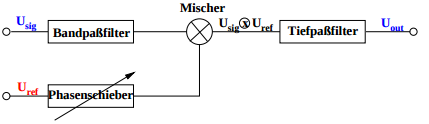
\includegraphics[width=0.8\textwidth]{V3033.png}
  \caption{Schematische Darstellung eines Lock-In-Verstärkers \cite{anleitung}}
  \label{fig:V3033}
\end{figure}\\
In Abbildung \ref{fig:V3034} sind die Signalverläufe für eine sinusförmige
Signalspannung zu sehen, wie sie auch in diesem Versuch vorkommen. Die
Signalspannung ist dabei
\begin{equation}
  U_\mathup{sig}\,=\,U_0\,\sin({\omega\,t})
  \label{eqn:1}
\end{equation}
Diese wird durch eine Rechteckspannung $U_\mathup{ref}$ derselben Spannung moduliert.
$U_\mathup{ref}$ ist dabei ein Schalter oder ein Chopper. Sie kann durch
eine Fourierreihe genähert werden. Dann erhält man aus dem Produkt von $U_\mathup{sig}$ und $U_\mathup{ref}$
\begin{equation}
  U_\mathup{out}\,=\,\frac{2}{\pi}U_0
  \label{eqn:2}
\end{equation}
Mit einer Phasendifferenz $\phi$ zwischen Nutz- und Referenzspannung wird
\ref{eqn:2} zu
\begin{equation}
  U_{out}\,=\,\frac{2}{\pi}U_0\cos(\phi)
  \label{eqn:3}
\end{equation}
Da die Cosinus-funktion maximal wird, wenn das Argument 0 (oder einem Vielfachen
von $2\,\pi$) entspricht, wird die Ausgangsspannung maximal für $\phi$\,=\,0,
also wenn es keinen Phasenunterschied zwischen Nutz- und Referenzspannung gibt.
\clearpage
\begin{figure}[htb]
  \centering
  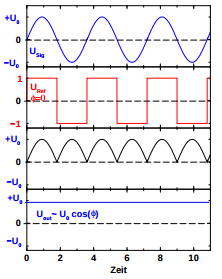
\includegraphics[width=0.5\textwidth]{V3034.png}
  \caption{Signalverläufe für eine sinusförmige Signalspannung \cite{anleitung}}
  \label{fig:V3034}
\end{figure}
\section{Durchführung}
\label{sec:durchführung}
\subsection{Versuchsaufbau}
\label{sec:aufbau}
In Abbildung \ref{fig:V3031} ist der Schaltplan eines Lock-In-Verstärkers zu
sehen. Als erstes wurde dieser Schaltplan aufgebaut. Der Schaltplan eines
Lock-In-Verstärkers beinhaltet einen Vorverstärker, die Hoch-, Tief-, und
Bandpassfilter, einen Phasenschieber, einen Funktionsgenerator, einen Rauschgenerator,
einen Tiefpass-Verstärker und einen Amplituden-/Lock-In-Detektor.
All diese Geräte sind seperat bedienbar. Dabei verstärkt der Vorverstärker das
zu untersuchende Signal. Die Filter sind dafür da, die gewünschten Frequenzen
aus dem Signal herausszufiltern. Mit dem Phasenschieber kann man das bereits in
der Theorie erwähnte $\phi$ variieren. Der Funktionsgenerator wird zum Erzeugen
periodischer elektrischer Signale genutzt. Der Rauschgenerator erzeugt Rauschen
als zufällige Signalschwankung.
\begin{figure}[htb]
  \centering
  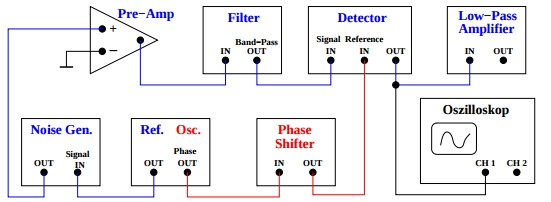
\includegraphics[width=0.9\textwidth]{V3031.png}
  \caption{Schaltplan eines Lock-In-Verstärkers \cite{anleitung}}
  \label{fig:V3031}
\end{figure}
\subsection{Versuchsdurchführung}
\label{sec:versuchsdurchführung}
Zuerst werden Messungen ohne Rauschsignal aufgenommen. Dabei wird der
Noise-Generator noch nicht eingeschaltet. Als nächstes wird ein Sinussignal $U_\mathup{sig}$
erzeugt mit \SI{1}{kHz} und \SI{20}{mV}. Dabei entsteht auch ein Referenzsignal
$U_\mathup{ref}$ mit gleicher Frequenz wie $U_\mathup{sig}$.\\ Die Ausgangsspannung $U_\mathup{out}$,
nach Integration durch den Tiefpass, wird 8 mal in Abhängigkeit von der Phasenverschiebung
bestimmt. Danach wird der Noise-Generator eingeschaltet und die Messungen wiederholt.

Als letztes wird noch ein Photo-Detektor in den Schaltplan integriert. Dieser
Schaltplan ist in \ref{fig:V3032} zu sehen. Die LED des Photo-Detektors blinkt
mit \SI{200}{Hz}. Sie kann mit einer Reckteckspannung moduliert werden.
Dann wird als Funktion des Abstandes zwischen LED und Photodiode die
Lichtintensität gemessen und der maximale Abstand $r_{max}$ bestimmt, bei dem
das Licht der LED die Photodiode noch erreicht.
Durch ein Oszilloskop werden die in der Auswertung genutzten Bilder gespeichert.
Dies ist mit Hilfe des "print"-Knopfes am Oszilloskop möglich.
Mit diesem Speicher-Oszilloskop können die Signale aller Komponenten einzeln
vermessen und skizziert werden.
\begin{figure}[htb]
  \centering
  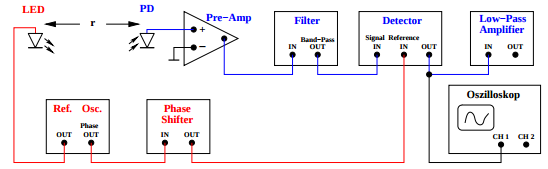
\includegraphics[width=0.8\textwidth]{V3032.png}
  \caption{Schaltplan eines Lock-In-Verstärkers mit einem Photo-Detektor \cite{anleitung}}
  \label{fig:V3032}
\end{figure}
\clearpage
\section{Auswertung}
\label{sec:auswertung}
\subsection{Messwerte}
Im laufe der drei Messreihen wurden folgende Werte gemessen:
\begin{table}
  \centering
  \caption{Ausgangsspannung vom Tiefpass bei der jeweiligen Phase in $\textdegree$.}
  \label{tab:Phasenverlauf}
  \sisetup{table-format=1.2}
  \begin{tabular}{S[table-format=3.0] S S}
    \toprule
     {Phase in $\textdegree$} & {Spannung bei inaktivem Noise Generator} & {Spannung bei aktivem Noise Generator} \\
    \midrule
    0 & 7.0 & 7.5 \\
    30 & 6.5 & 7.25 \\
    60 & 3.25 & 3.6 \\
    90 & 0.25 & 0.25 \\
    120 & -2.7 & -2.75 \\
    150 & -6.4 & -6.75 \\
    180 & -7.0 & -7.75 \\
    210 & -6.6 & -7.0 \\
    240 & -3.4 & -3.75 \\
    270 & -0.25 & -0.25 \\
    300 & 2.5 & 2.6 \\
    330 & 6.25 & 6.75 \\
    360 & 7.2 & 7.75 \\
    \bottomrule
  \end{tabular}
\end{table}
\begin{table}
  \centering
  \caption{Ausgangsspannung bei der Messung der Lichtintensität in Abhängigkeit vom Abstand.}
  \label{tab:Intens}
  \sisetup{table-format=3.1}
  \begin{tabular}{S[table-format=4.0] S[table-format=1.2] S}
    \toprule
    {Lock-In Gain} & {Spannung in $\si{\volt}$} & {Abstand in $\si{\centi\meter}$} \\
    \midrule
    10 & 8.5 & 6.1 \\
    10 & 3.5 & 11.1 \\
    10 & 2 & 16.1 \\
    10 & 1.25 & 21.1 \\
    50 & 4 & 26.1 \\
    50 & 2.75 & 31.1 \\
    50 & 2 & 36.1 \\
    50 & 1.75 & 41.1 \\
    200 & 3.5 & 46.1 \\
    200 & 2.6 & 51.1 \\
    200 & 2.25 & 56.1 \\
    200 & 2 & 61.1 \\
    500 & 2.5 & 66.1 \\
    1000 & 3.1 & 71.1 \\
    1000 & 2.9 & 81.1 \\
    1000 & 2.75 & 91.1 \\
    1000 & 2.6 & 101.1 \\
    1000 & 2.5 & 111.1 \\
    1000 & 2.4 & 121.1 \\
    1000 & 2.25 & 131.1 \\
    1000 & 2.2 & 141.1 \\
    \bottomrule
  \end{tabular}
\end{table}
\clearpage
\subsection{Messungen zur Phasendifferenz}
Zunächst war gefragt an welchem Ausgang des Ref./Oscil. man die Spannung variieren
kann und an welchem eine konstante Spannungsamplitude anliegt.\\
Antwort: An dem Ref.-Ausgang (Signal) kann man die Spannung variieren während am
Oscil.-Ausgang(Referenz) eine konstante Spannungsamplitude von ca. $\SI{30}{\volt}$
anliegt.
\\
Als nächstes wird die Apparatur schrittweise, bei inaktivem Noise Generator, aufgebaut.
Dabei entstanden die folgenden Bilder:
\begin{figure}[htb]
  \centering
  \begin{subfigure}{0.48\textwidth}
    \centering
    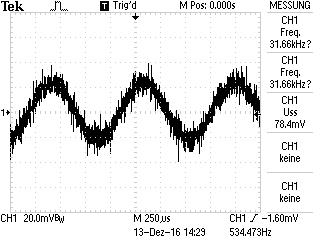
\includegraphics[width=\textwidth]{F0010TEK.jpg}
    \caption{Verlauf der Signalspannung.\\}
    \label{fig:1}
    \qquad
  \end{subfigure}
  \begin{subfigure}{0.48\textwidth}
    \centering
    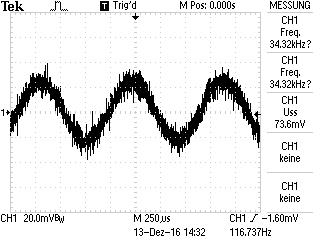
\includegraphics[width=\textwidth]{F0012TEK.jpg}
    \caption{Verlauf der Signalspannung am inaktiven Noise Generator abgenommen.}
    \label{fig:2}
    \qquad
  \end{subfigure}
\end{figure}
\begin{figure}[htb]
  \centering
  \begin{subfigure}{0.48\textwidth}
    \centering
    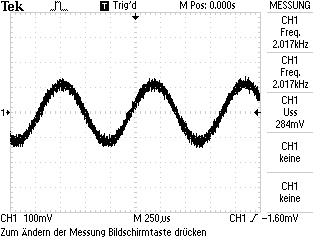
\includegraphics[width=\textwidth]{F0011TEK.jpg}
    \caption{Verlauf der Signalspannung nach\\ dem Durchlaufen des Vorverstärkers.}
    \label{fig:3}
    \qquad
  \end{subfigure}
  \begin{subfigure}{0.48\textwidth}
    \centering
    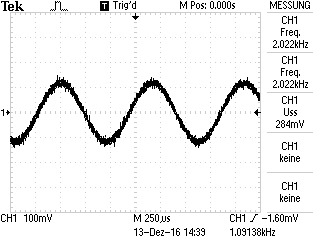
\includegraphics[width=\textwidth]{F0013TEK.jpg}
    \caption{Verlauf der Signalspannung nach\\ dem Filter.}
    \label{fig:4}
    \qquad
  \end{subfigure}
\end{figure}
\begin{figure}[htb]
  \centering
  \begin{subfigure}{0.48\textwidth}
    \centering
    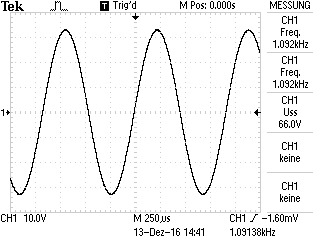
\includegraphics[width=\textwidth]{F0014TEK.jpg}
    \caption{Verlauf der Referenzspannung.}
    \label{fig:5}
    \qquad
  \end{subfigure}
  \begin{subfigure}{0.48\textwidth}
    \centering
    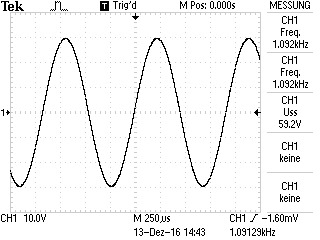
\includegraphics[width=\textwidth]{F0015TEK.jpg}
    \caption{Verlauf der Referenzspannung am Ausgang des Phasenverschiebers.}
    \label{fig:6}
    \qquad
  \end{subfigure}
\end{figure}\\
\\
\\
\\
\\
\\
Als nächstes sollten mindestens 5 Bilder von verschiedenen Phasendifferenzen gemacht werden:
\begin{figure}[htb]
  \centering
  \begin{subfigure}{0.48\textwidth}
    \centering
    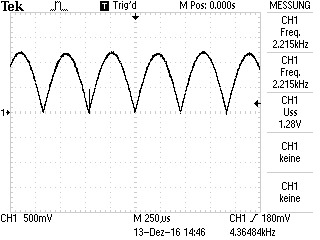
\includegraphics[width=\textwidth]{F0016TEK.jpg}
    \caption{Spannungsverlauf am Lock-In Detektor\\ bei gleicher Phase von Signal und Referenz.}
    \label{fig:7}
    \qquad
  \end{subfigure}
  \begin{subfigure}{0.48\textwidth}
    \centering
    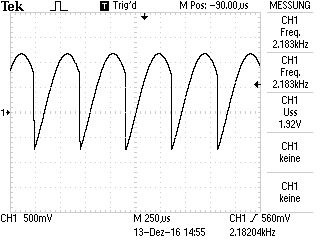
\includegraphics[width=\textwidth]{F0018TEK.jpg}
    \caption{Spannungsverlauf bei einer Phasendifferenz von 45°.}
    \label{fig:8}
    \qquad
  \end{subfigure}
\end{figure}
\begin{figure}[htb]
  \centering
  \begin{subfigure}{0.48\textwidth}
    \centering
    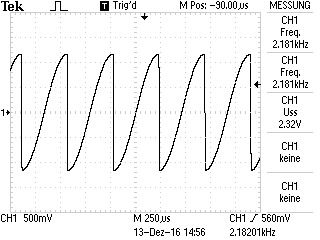
\includegraphics[width=\textwidth]{F0019TEK.jpg}
    \caption{Spannungsverlauf bei einer\\ Phasendifferenz von 90°.}
    \label{fig:9}
    \qquad
  \end{subfigure}
  \begin{subfigure}{0.48\textwidth}
    \centering
    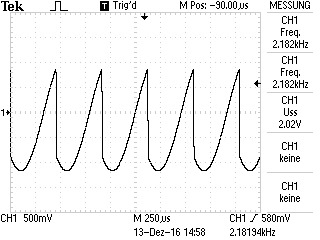
\includegraphics[width=\textwidth]{F0020TEK.jpg}
    \caption{Spannungsverlauf bei einer\\ Phasendifferenz von 135°.}
    \label{fig:10}
    \qquad
  \end{subfigure}
\end{figure}
\begin{figure}[htb]
  \centering
  \begin{subfigure}{0.48\textwidth}
    \centering
    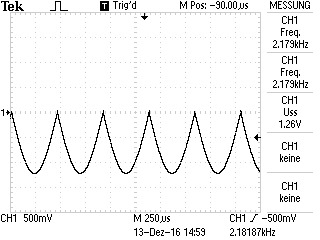
\includegraphics[width=\textwidth]{F0021TEK.jpg}
    \caption{Spannungsverlauf bei einer\\ Phasendifferenz von 180°.}
    \label{fig:11}
    \qquad
  \end{subfigure}
  \begin{subfigure}{0.48\textwidth}
    \centering
    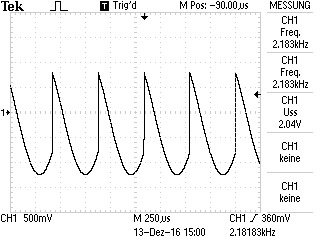
\includegraphics[width=\textwidth]{F0022TEK.jpg}
    \caption{Spannungsverlauf bei einer\\ Phasendifferenz von 225°.}
    \label{fig:12}
    \qquad
  \end{subfigure}
\end{figure}
\begin{figure}[htb]
  \centering
  \begin{subfigure}{0.48\textwidth}
    \centering
    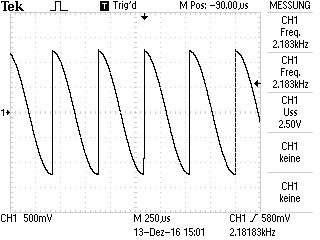
\includegraphics[width=\textwidth]{F0023TEK.jpg}
    \caption{Spannungsverlauf bei einer\\ Phasendifferenz von 270°.}
    \label{fig:13}
    \qquad
  \end{subfigure}
  \begin{subfigure}{0.48\textwidth}
    \centering
    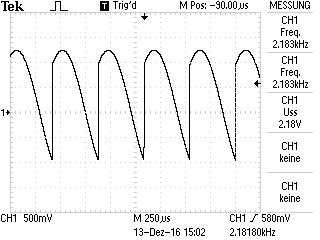
\includegraphics[width=\textwidth]{F0024TEK.jpg}
    \caption{Spannungsverlauf bei einer\\ Phasendifferenz von 315°.}
    \label{fig:14}
    \qquad
  \end{subfigure}
\end{figure}
\clearpage
Nun werden Bilder von den Spannungsverläufen, bei eingeschaltetem Noise Generator, gemacht:
\begin{figure}[htb]
  \centering
  \begin{subfigure}{0.48\textwidth}
    \centering
    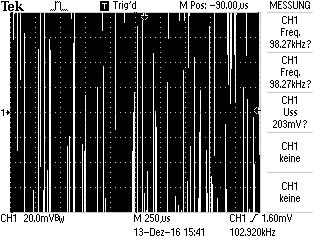
\includegraphics[width=\textwidth]{F0026TEK.jpg}
    \caption{Signalspannung mit dem durch den\\ Noise Generator erzeugten Rauschen.}
    \label{fig:15}
    \qquad
  \end{subfigure}
  \begin{subfigure}{0.48\textwidth}
    \centering
    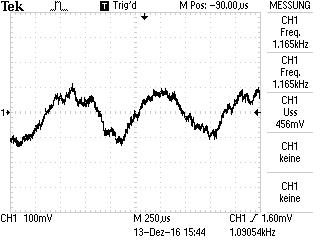
\includegraphics[width=\textwidth]{F0027TEK.jpg}
    \caption{Signal nach der Filterung.}
    \label{fig:16}
    \qquad
  \end{subfigure}
\end{figure}
\begin{figure}[htb]
  \centering
  \begin{subfigure}{0.48\textwidth}
    \centering
    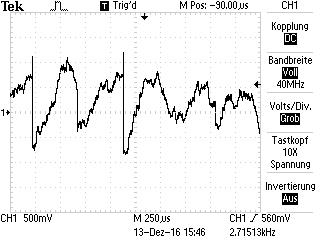
\includegraphics[width=\textwidth]{F0028TEK.jpg}
    \caption{Spannungsverlauf am Ausgang des\\ Lock-In Detektors bei gleicher Phase\\ zum Referenzsignal.}
    \label{fig:17}
    \qquad
  \end{subfigure}
  \begin{subfigure}{0.48\textwidth}
    \centering
    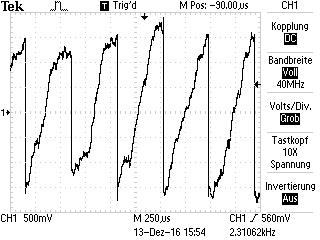
\includegraphics[width=\textwidth]{F0029TEK.jpg}
    \caption{Spannungsverlauf bei einer\\ Phasendifferenz von 90°.}
    \label{fig:18}
    \qquad
  \end{subfigure}
\end{figure}
\begin{figure}[htb]
  \centering
  \begin{subfigure}{0.48\textwidth}
    \centering
    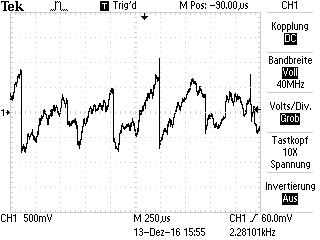
\includegraphics[width=\textwidth]{F0030TEK.jpg}
    \caption{Spannungsverlauf bei einer\\ Phasendifferenz von 180°.}
    \label{fig:19}
    \qquad
  \end{subfigure}
  \begin{subfigure}{0.48\textwidth}
    \centering
    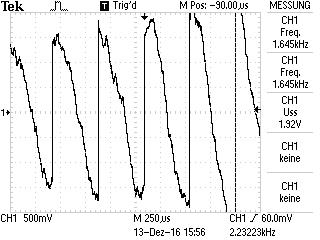
\includegraphics[width=\textwidth]{F0031TEK.jpg}
    \caption{Spannungsverlauf bei einer\\ Phasendifferenz von 270°.}
    \label{fig:20}
    \qquad
  \end{subfigure}
\end{figure}
\\
\\
\\
\\
\\
\\
\\
\\
\\
\\
Die Augangsspannung am Tiefpass wird für beide Messreihen gegen die Phasendifferenz
aufgetragen und durch Python mit einer Funktion der Form
\begin{equation}
  U = a \cdot \cos \left( \phi + b \right)
  \label{eqn:fit1}
\end{equation}
gefittet.

Für die Messreihe zum inaktiven Noise Generator ergeben sich als Parameter $a = 7.1 \pm 0.2$
und $b = -0.05 \pm 0.02$, während sich für die Messreihe zum aktiven Noise Generator $a = 7.6 \pm 0.2$
und $b = -0.06 \pm 0.02$ ergeben.
\begin{figure}
  \centering
  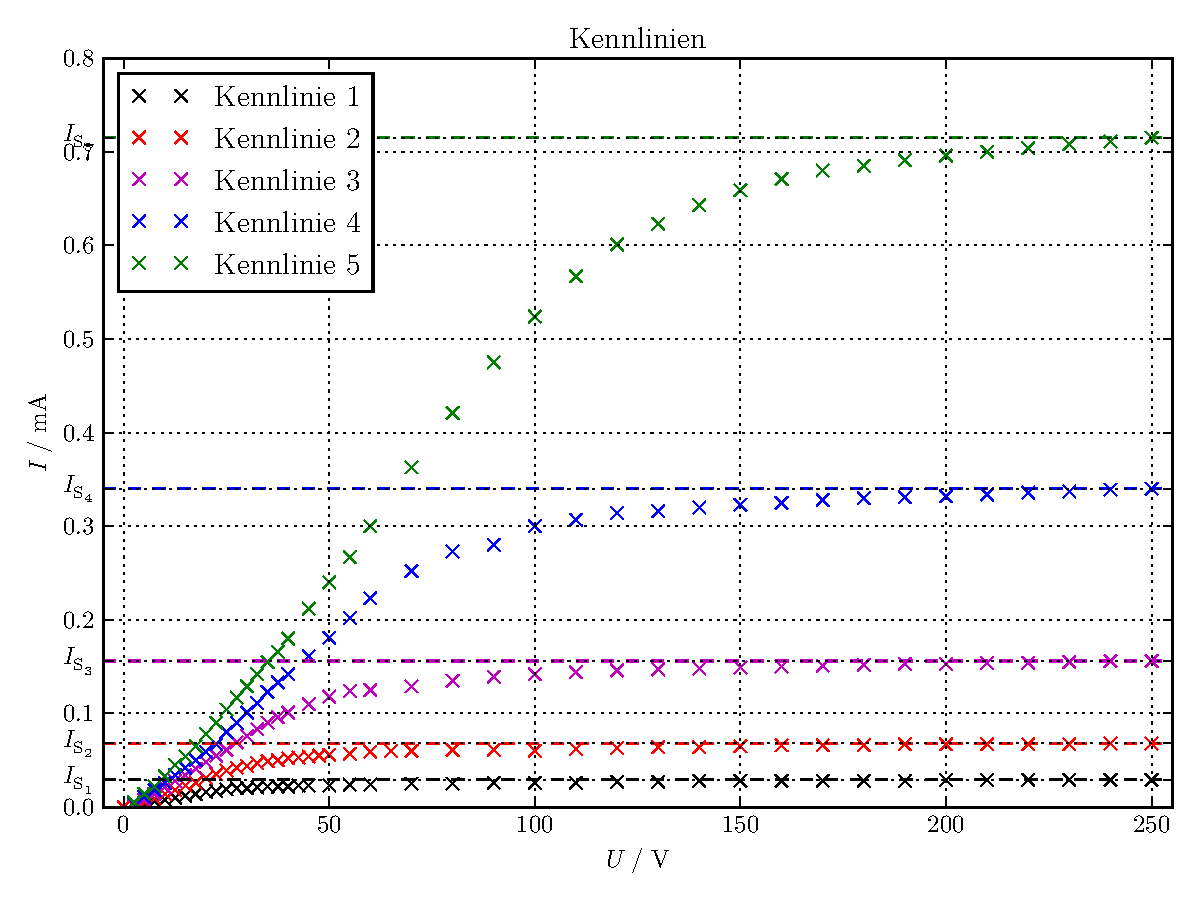
\includegraphics[width=0.70\textwidth]{Plot.pdf}
  \caption{Graph der Messwerte und der Fitfunktion bei inaktivem Noise Generator.}
  \label{fig:plot1}
\end{figure}
\clearpage
\begin{figure}
  \centering
  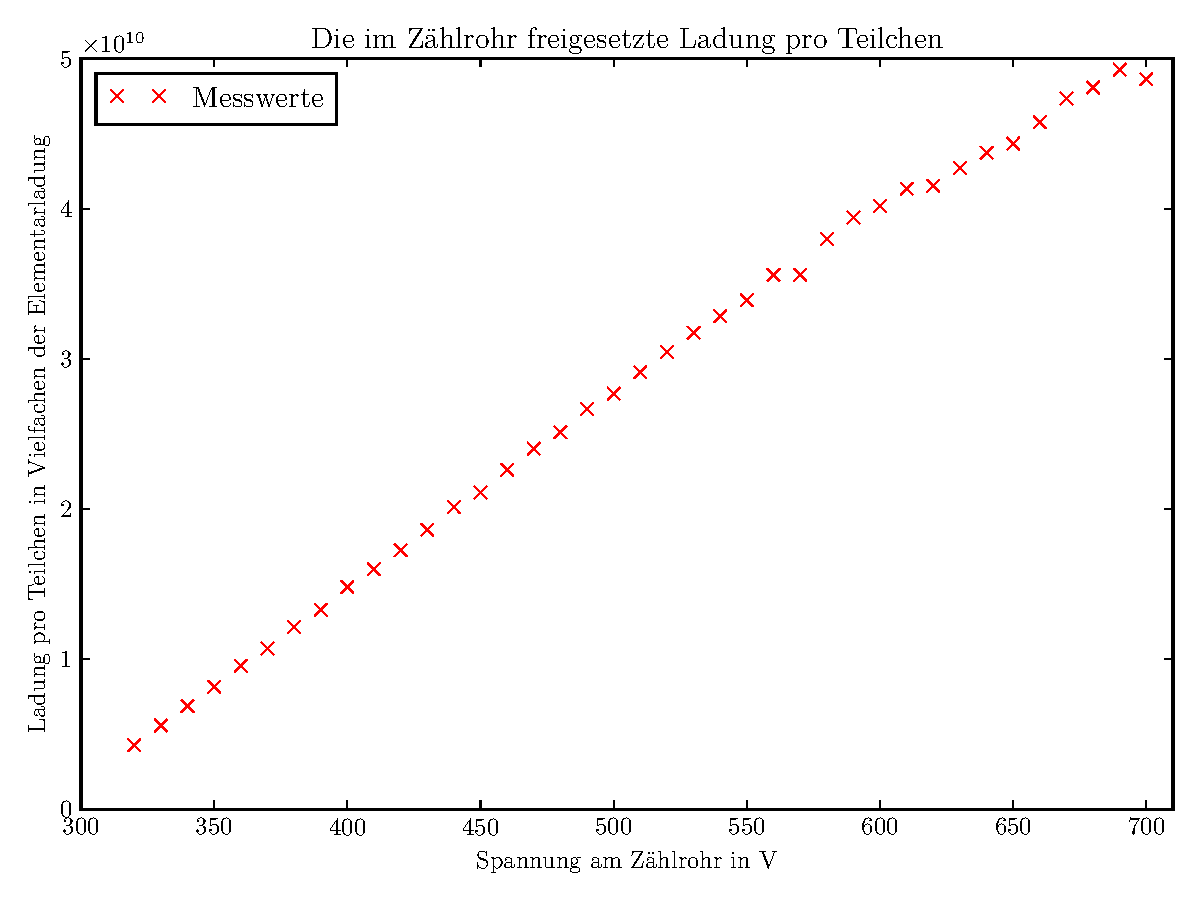
\includegraphics[width=0.80\textwidth]{Plot2.pdf}
  \caption{Graph der Messwerte und der Fitfunktion bei aktivem Noise Generator.}
  \label{fig:plot2}
\end{figure}
Demnach folgt aus $b$ eine interne Phasenverschiebung des Gerätes von $3 \textdegree$.
\subsection{Messungen zur Lichtintensität}
Zur Messung der Lichtintensität in Abhängigkeit vom Abstand wird der Logarithmus
vom Betrag der gemessene Spannung gegen den Logarithmus vom Betrag des Abstands
aufgetragen und mit einer linearen Funktion
\begin{equation}
  g \left( x \right) = b \cdot x + a
  \label{eqn:fit}
\end{equation}
gefittet.
Dabei ergeben sich die Parameter zu: $b =  \num{-2.18(9)}$ und $a = \num{-3.5(1)}$.
Mit $b$ lässt sich erkennen, dass die Spannung mit dem Abstandsquadrat abnimmt.
Der folgende Graph zeigt den Verlauf dieser Funktion aufgetragen.
\clearpage
\begin{figure}
  \centering
  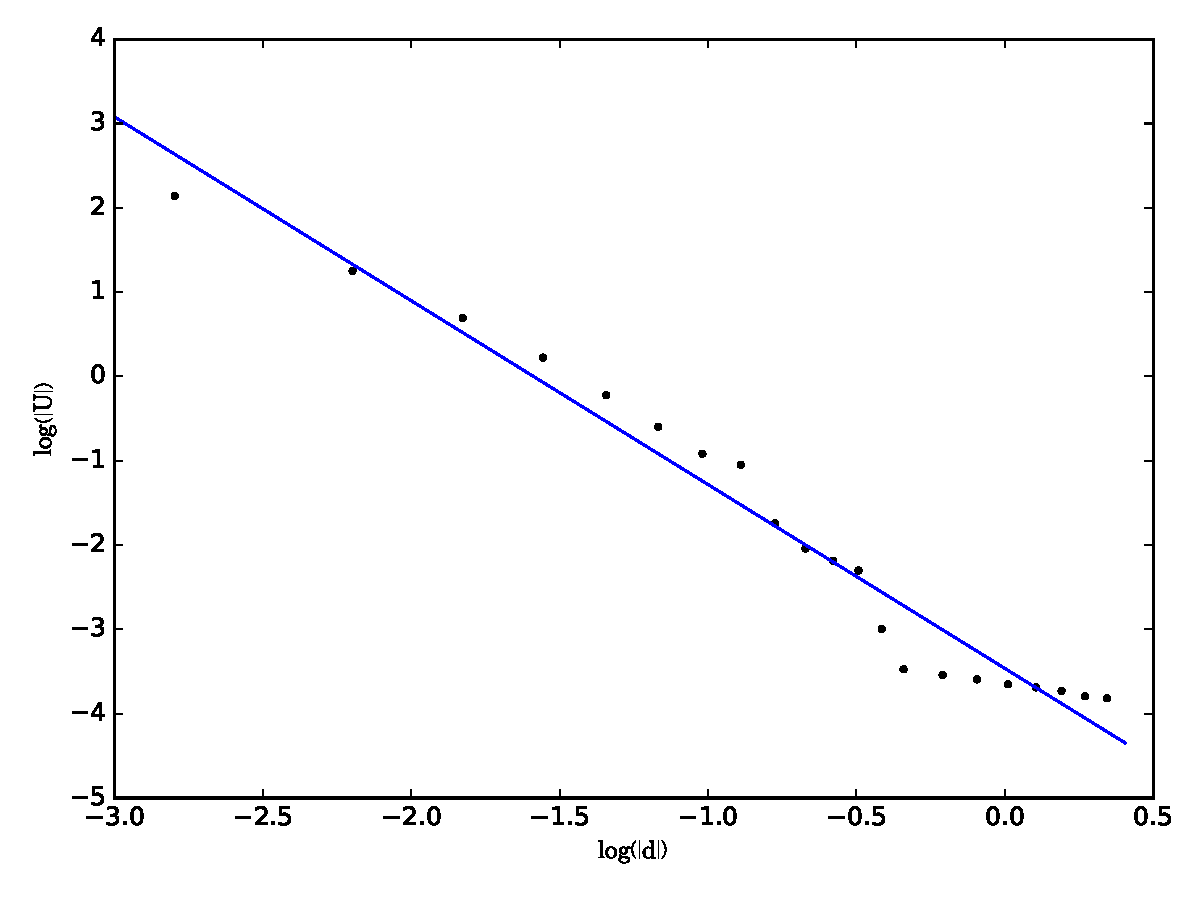
\includegraphics[width=0.80\textwidth]{licht-messung.pdf}
  \caption{Graph der Messwerte und der Fitfunktion bei der Messung der Lichtintensität.}
  \label{fig:plot3}
\end{figure}
Wie man sieht wird die Messung ab einer Distanz von $\SI{50}{\centi\meter}$ relativ
ungenau. Somit lässt sich bis dorthin eindeutig das Signal der LED nachweisen.
Auf größere Entfernung nimmt das Signal weiterhin ab, wobei des sich bei einer Distanz
von $\SI{1}{\meter}$ allmählich asymptotisch einem konstanten Wert nähert.
\newpage
\section{Diskussion}
\label{sec:diskussion}

Anhand der drei Messreihen lässt sich gut die Funktionsweise des Lock-In Verstärkers
erkennen. Das Signal, welches in der ersten Messreihe untersucht wurde enthielt
schon ein leichtes Rauschen, welches fast gänzlich verschwand. Gut zu erkennen war
dabei, dass das Referenzsignal immer entsprechend der Phasenverschiebung einen 180°
breiten Abschnitt des Sinussignals ausschneidet und mit doppelter Frequenz darstellt,
was an dem Vorzeichen der Referenzspannung liegt.
Nach dem einschalten des Noise Generators war das Signal nicht mehr zu erkennen,
doch erhält man am Ende fast die gleichen Werte, wie bei der ersten Messreihe.

Auch bei der dritten Messreihe war das Gerät in der lage das LED Signal zu identifizieren.
Dass es sich hierbei um das Signal der LED handelt, kann man anhand der $\frac{1}{r^{2.18}}$
Abhängigkeit erahnen. Im Idealfall nimmt die Lichtintensität mit $\frac{1}{r^2}$ ab.
Jene Abweichung lässt sich damit begründen, dass sowohl die LED als auch die Photodiode
um die vertikale Achse drehbar sind. Somit führt eine Ungenauigkeit in der Ausrichtung
dieser beiden Geräte dazu, dass man mit zunehmender Distanz einen zusätzlichen
Einfluss durch den von der direkten verbindungslinie abweichend schwächer werdenden
Lichtkegel der LED erhält.

Ein weiterer Faktor, der möglicherweise eine Rolle spielt ist die Deckenbeleuchtung,
die mit einer Frequenz von $\SI{50}{\hertz}$ leuchtet und mit $\SI{100}{\hertz}$ in
dem Lock-In Verstärker ankommt. Normalerweise sollte eben jenes Licht durch den Lock-In
Verstärker herausgefiltert werden, doch konnte man, z.B. wenn man eine Hand in den
Lichtweg der LED hält, immernoch eine Spannung von $\SI{0.02}{\volt}$ messen. Möglicherweise
könnte es zu einem derartigen Einfluss kommen, da $\SI{200}{\hertz}$ ein Vielfaches
von $\SI{100}{\hertz}$ ist und dies somit je nach Phasendifferenz zum Referenzsignal
für eine kleine Spannung sorgen könnte. Des weiteren fällt auf, dass die gemessene Spannung
bei der dritten Messreihe bei jedem umstellen des Gains einen kleinen Sprung nach unten macht.
\nocite{*}
\printbibliography

\end{document}
